\chapter{Reverse Engineering Bayesian Computations from Spike Trains}
\label{chap:nine}

The preceding chapters have developed a range of probabilistic models
for neural spike trains that leverage our intuitions about neural
types, features, and states to inform structured prior distributions over
the dynamics of neural activity. In this chapter, we take a
first step toward reconciling these intuitive models with the host of
theoretical models of neural computation. From a Bayesian perspective,
theoretical models can be seen as prior distributions on activity ---
albeit highly sophisticated ones. By connecting theory to observation
in a hierarchical probabilistic model, we provide the link
necessary to test, evaluate, and revise our theories in a
data-driven fashion.
As an exercise in meta-reasoning, the theory we test with this
Bayesian approach is that neural populations are themselves performing
Bayesian inference.

This chapter is organized as follows.  First, in
Section~\ref{sec:bayesian_brain} we briefly review the ``Bayesian
brain'' hypothesis, the various lines of evidence supporting this
hypothesis, and some of the suggestions of how neurons could represent
probability distributions and carry out Bayesian calculations.  Then,
in Section~\ref{sec:representation} we present a distributed representation
scheme, and in Section~\ref{sec:complexity} we provide a novel
analysis of its complexity in the spirit of
\citet{valiant1994circuits}. This which provides important constraints
on biological plausibility of this scheme and the number of neurons we
must observe in order to test this theory.
Section~\ref{sec:inference} adapts existing theories to show how
neural circuits could perform mean-field variational inference in a
restricted class of graphical models given our representation scheme.
A simple example of inference in a mixture model is illustrated in
Section~\ref{sec:mixture_example}.  Finally, in
Section~\ref{sec:reverse_engineering} we show that the dynamics of
inference in this model are equivalent to a nonlinear autoregressive model
with weights drawn from a stochastic block model, thus providing a
``top-down,'' theoretical justification for the intuitive models
developed in Chapter~\ref{chap:five}.  With this insight, we show how
simple probabilistic models can be reverse engineered from spike
trains using Bayesian inference and a
Bayesian theory of neural computation. Section~\ref{sec:future}
considers some important open problems and directions for future work.


\section{The ``Bayesian Brain'' Hypothesis}
\label{sec:bayesian_brain}
Bayesian theories of neural computation address a fundamental
question: how do organisms reason, act, and make decisions given only
limited, noisy information about the world around them?  Bayes' rule
tells us how an optimal agent should combine noisy information with
prior knowledge to make inferences and decisions under uncertainty.
That the brain may employ or approximate Bayesian methods is an idea
that dates back as far as \citet{helmholtz1925treatise}.  At the
cognitive level, Bayesian models have proven extraordinarily useful
for understanding and explaining human and animal
behavior~\citep{tenenbaum2011grow, griffiths2008bayesian}. These
cognitive models span a variety of domains, from lower level systems
like visual perception~\citep{knill1996perception,
  brainard1997bayesian, weiss2002motion, yuille2006vision,
  Stocker2006, Simoncelli2009} and motor control~\citep{Kording2004} to
higher level systems of sensory integration~\citep{ernst2002humans},
time interval estimation~\citep{jazayeri2010temporal}, 
language processing~\citep{chater2006probabilistic},
attention~\citep{whiteley2012attention, chikkerur2010,
  dayan2010selective}, and learning~\citep{tenenbaum2006theory,
  courville2006bayesian} The success of these models in explaining
behavior suggests that the brain may be performing, or at least
approximating, Bayesian computations.

Further buttressing the Bayesian brain hypothesis, some experiments
have shown Bayes-optimal behavior along with simultaneous neural responses
that are strongly correlated with relevant probabilistic quantities.
For example, \citet{Yang2007} trained monkeys to make an eye movement
to either the left or the right based on an observed set of shapes.
Each shape contributed an additive ``weight'' to the log probability
that reward would be given for leftward movements rather than
rightward, so the optimal strategy (once the weights were
learned) was to sum the weights, compute the log probability of left
versus right, and choose the direction most likely to yield a
reward.  In effect, the monkeys had to perform inference in a simple
mixture model. The monkeys learned to perform this task optimally, and
\citet{Yang2007} found that the firing rates of neurons in parietal
cortex were proportional to the log likelihood ratio of left versus
right. While it is possible that the monkeys simply learned a
discriminative mapping from shapes to decisions, subsequent work
showed that when the paradigm was extended to allow the monkey to
opt-out of making a decision and obtain a smaller but guaranteed
reward, the monkey chose to opt out only when the probability of
left versus right was below a threshold \citep{Kiani2009}.

Further evidence of neural probabilistic inference has been found in
other simple tasks. In a time interval reproduction task, non-human
primates exhibited behavior consistent with a Bayesian model, and
simultaneous recordings in parietal cortex found that some neurons
encoded interval estimates that could support this behavior
\citep{jazayeri2015neural}. In another line of work, neural correlates
of multisensory cue integration were found in macaque monkeys
performing a heading discrimination task. These neurons combined both
visual and vestibular inputs in a manner consistent with Bayesian
theory \citep{gu2008neural, morgan2008multisensory, fetsch2009dynamic,
  fetsch2012neural}.  While these experiments provide some compelling
evidence in favor of a simple probabilistic computations in neural
circuits, there is a large gap between these experiments and the rich
array of cognitive phenomena surveyed above. To bridge this gap, we
need a broader theory of Bayesian inference in neural circuits, and
more powerful tools to link these theories to neural activity.

The past decade has witnessed a surge of interest in theoretical
models of Bayesian inference with spiking neurons, and this work has
been the subject of a number of recent surveys~\citep{Simoncelli2009,
  fiser2010statistically, pouget2013probabilistic, ma2014neural}.
These theories can be broadly characterized by their answers to three
successive questions:
\begin{enumerate}
\item How are probabilities are represented, and how are the conditional
  probability distributions that constitute the probabilistic model
  encoded?
\item Given a representation, how do neural dynamics compute the
  desired posterior distribution? In other words, what is the
  algorithm of probabilistic inference, and how is it reified in a
  population of neurons? These dynamics must respect the natural
  constraints of neural systems, for example, that neural connectivity
  is sparse and that neurons have limited computational power.
\item Finally, how are the parameters of the probabilistic model
  learned, and how are new variables of interest incorporated into
  an existing model?
\end{enumerate}
% Direct vs Log vs Leveraging neuronal variability vs Predictive coding
The simplest and most common answer to the first question is that
neural firing rates are proportional to probability~\citep{Hinton1983,
  Hinton1992, Anderson1994, Barber2003, Buesing2011, Berkes2011,
  nessler2013bayesian, legenstein2014ensembles} or some function of
the probability, like its log~\citep{Rao2004, beck2007exact, Rao2007,
  litvak2009cortical}. Others have suggested that probability
distributions are encoded implicitly by the stochasticity of neurons
\citep{Zemel1998, Sahani2003, Ma2006}. Still others have contended that
neurons employ a predictive coding scheme to convey probabilistic
information~\citep{Rao1999, Deneve2008a, Huang2011}.  An interesting
alternative deserving of more attention is that distributions may be
implicitly encoded in the number of neurons representing a particular
value or, similarly, in the width of neural tuning
curves~\citep{Shi2009, Ganguli2010}. 

% Exact, Belief Propagation, Variational inference, importance sampling,
% MCMC, particle filtering
Along with this host of representational hypotheses has come an
equally broad set of proposed inference algorithms. 
% Typically, these
% proposals are tied to a specific assumption about representation.  
In
the simplest models, like mixture models with a single latent
variable, inference can be performed exactly in a single step.  For
more complicated models, some dynamic and often approximate inference 
algorithm is necessary. Of these, belief propagation and related
message passing algorithms~\citep{Rao2007, litvak2009cortical},
variational inference \citep{Friston2010, nessler2013bayesian},
and sampling based methods like Markov chain Monte Carlo (MCMC)
\citep{hoyer2003interpreting, Buesing2011, 
  Berkes2011, gershman2012multistability, legenstein2014ensembles},
Hamiltonian Monte Carlo~\citep{aitchison2014hamiltonian},
importance sampling~\citep{Shi2009}, 
and particle filtering \citep{lee2003hierarchical} have
all been suggested. This amazing diversity speaks to both the
computational power of neural populations as well as the
enormous challenge in winnowing the field of contending theories.

% Learning via maximization of variational lower bound, synaptic sampling
The question of learning has received less attention; indeed, many
theories have ignored it completely. Those that have addressed it tend to
equate learning with synaptic plasticity. In some cases, synaptic
plasticity rules like spike-timing dependent plasticity can be seen as
maximizing a lower bound on the marginal log likelihood
\citep{Friston2010, nessler2013bayesian, rezende2011variational}. In
others, the stochasticity of synapses (e.g. stochastic vesicle
release) is seen as sampling from a distribution over weights
\citep{aitchison2015synaptic, kappel2015synaptic, kappel2015network, tully2014synaptic}.
These theories address unsupervised learning of model parameters, but
the larger question of learning model structure, via either supervised
or unsupervised means, remains largely a mystery.


Given the breadth and depth of existing theories of neural inference,
our intention here is not to present a radically novel
theory. Instead, our focus is on how we may assess the viability of a
theory of neural inference. To that end, we provide a detailed
description of a distributed representation of probability, analyze
its complexity, show how inference could be performed with this representation,
and provide a simple example of how this representation could be
reverse engineered from neural spike train recordings. 

%Then weanalyze the complexity of this representational scheme in terms of the
%support of the distribution, number of neurons, integration time,
%firing rate, and degree of connectivity required to represent a
%distribution with both low error and high confidence, in the spirit of
%\citet{valiant1994circuits, valiant2005memorization}.  As shown
%by~\citet{gao2015simplicity}, these complexity-theoretic analyses
%inform our assessment of the biological plausibility of the theory, as
%well as the number of neurons we must measure in order to test the
%theory. Given this representation, we show how Bayesian inference can
%be performed in a subset of probabilistic models using mean-field
%variational inference. Then, we show how the dynamics of inference
%correspond to exactly the generalized linear model dynamics studied in
%Chapter~\ref{chap:gfive}, thereby enabling us to use those tools to reverse engineer
%a probabilistic model from a neural spike train recording.  In the
%closing discussion, we consider how these techniques could be extended
%beyond the relatively simple theory of inference studied here.

\section{A Direct Distributed Representation of Probability Distributions}
\label{sec:representation}


\sloppy
As described above, the simplest representation of probability is a \emph{direct}
representation in which neural firing rates reflect instantaneous
probabilities. Assume a population of neurons is responsible for
representing the distribution over values that a set of random
variables may take on. We denote this set of variables 
by,~${\bz = \{z_1, \ldots, z_J\}}$.  For
simplicity, assume for now that these variables can only assume a
discrete set of values,~${\{1, \ldots, K\}}$.  Our
neural population is thus tasked with representing probability
vectors,~$\bpi^{(j)}$, for each 
variable. The entries of these vectors are,~${\pi^{(j)}_k = \Pr(z_j=k)}$.
In Section~\ref{sec:future}, we discuss how this representation could
be extended to continuous probability density functions by assigning
each neuron a basis function or tuning curve over the support of the
distribution, as in~\citet{Barber2003, Ma2006, beck2007exact}. 

In a \emph{distributed} representation, each variable-value
pair,~$(z_j,k)$, is associated with a subpopulation of~$R$
neurons. This is inspired by \citet{valiant1994circuits,
  valiant2005memorization}, and is similar to the ensemble based
neural sampling code of \citet{legenstein2014ensembles}.  We further
assume that these subpopulations are \emph{non-overlapping} such that
each neuron can be represented with at most one variable-value pair.
Let~${j_n \in \{1, \ldots, J\}}$ denote the index of the specific
variable and~$k_n \in \{1, \ldots K\}$ denote the particular
value that neuron~$n$ represents.
%A representation size of~$R$ implies that~$\sum_{n=1}^N \bbI[j_n=h] \, \bbI[k_n=k] = R$.


% Figure: Example of neural inference in a simple mixture model
\begin{figure}[t!]
  \centering
  \begin{subfigure}[b]{1.6in}
    \centering
    \caption{}
    \vspace{-.3in}
    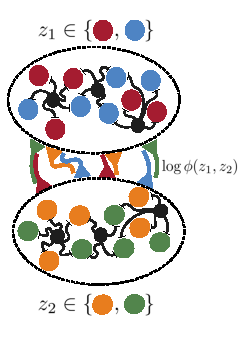
\includegraphics[width=\textwidth]{figures/ch9/example_population.pdf}
    \label{fig:representation_population}
  \end{subfigure}
  \begin{subfigure}[b]{1.9in}
    \centering
    \caption{}
    \vspace{-.3in}
    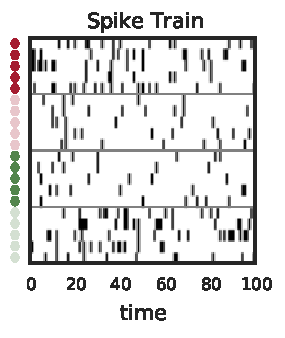
\includegraphics[width=\textwidth]{figures/ch9/example_spiketrain}
    \label{fig:representation_spiketrain}
  \end{subfigure}
  \begin{subfigure}[b]{1.8in}
    \centering
    \caption{}
    \vspace{-.3in}
    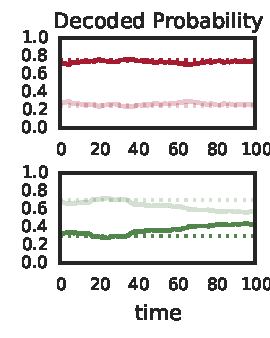
\includegraphics[width=\textwidth]{figures/ch9/example_prs}
    \label{fig:representation_prs}
  \end{subfigure}
  \vspace{-.25in}
  \caption[Example of a population of neurons encoding a probability
    distribution] {Example of a population of neurons encoding marginal
    probability distributions for two binary random variables,~$z_1$
    and~$z_2$. Each variable is represented by a population of neurons,
    which is further divided into subpopulations for each value the variable
    can take on. In~\textbf{(a)},~$z_1$ is represented by red neurons, with
    dark red neurons representing~${z_1=1}$ and light red representing~${z_1=0}$.
    Interneurons (black) provide normalization in the form of local inhibition.
    Excitatory connections between populations implement probabilistic inference.
    \textbf{(b)} The population spike train encodes the marginal distributions.
    For example,~${\Pr(z_1=1)}$ is proportional to the spike count of the subpopulation
    of dark red neurons.
    \textbf{(c)} These probabilities are decoded by integrating
    spike counts for each subpopulation over time and normalizing across
    subpopulations for each variable. Dotted lines: true probability. 
  }
 \label{fig:representation}
\end{figure}



Now let~$s_{t,n}$ denote the number of spikes fired by neuron ~$n$ in
the~$t$-th time bin. The relative spike counts encode instantaneous
probability distributions for each variable.  If neurons representing
a particular value fire twice as many spikes as neurons representing a
competing value, then the first value is twice as likely. We introduce
the notion of an \emph{integration time},~$T_I$, over which spikes are
counted to estimate the probability distribution. With this notation,
the empirical distribution,~$\widehat{\bpi}_t^{(j)}$, is defined by,
\begin{align*}
  \widehat{\pi}_{t,k}^{(j)} &=
  \frac{\sum_{\Delta = 1}^{T_I} \sum_{n=1}^N \bbI[j_n=j, k_n=k] \, s_{t-\Delta,n}}
       {\sum_{\Delta = 1}^{T_I} \sum_{n=1}^N \bbI[j_n=j] \, s_{t-\Delta,n}}.
\end{align*}
The numerator counts spikes from neurons representing the particular value,~$z_j=k$;
the denominator counts all spikes from neurons representing~$z_j$.


We assume these neurons are stochastic, each endowed
with an instantaneous firing rate,~$\lambda_{t,n}$, which gives rise to an
instantaneous spike count,~$s_{t,n}$ according to a Poisson distribution,
${
s_{t,n} \sim \distPoisson(\lambda_{t,n}).
}$
Thus, while the firing rate may encode one distribution, the distribution
that is read out from a finite number of spikes will differ. 

To summarize, the direct distributed representation entails the following
assumption:

\begin{assumption}
  Neurons represent discrete probability distributions with a direct,
  distributed code. Each variable-value pair is allotted~$R$ neurons
  that emit spikes according to a Poisson distribution.
  Spikes are integrated over the subpopulation and over an integration
  time window,~$T_I$, to obtain an unnormalized probability for the
  variable-value pair. By normalizing across subpopulations, they decode
  the probability distribution. 
\end{assumption}

\section{Complexity of the Direct Distributed Representation}
\label{sec:complexity}

In pioneering work, \citet{valiant1994circuits} suggested that
the tools of computational learning theory, which provide
rigorous computational limits on statistical learning, may
apply equally well to learning in biological systems. All
that is needed is a model of biological computation and a
precisely stated learning algorithm. If the resources
required by this algorithm (e.g. number of neurons or spikes)
grow exponentially quickly with the size of learning problem,
then it is highly unlikely that the algorithm is employed
by the brain. In other words, biology is bound by the same
limits of computational tractability as our silicon devices,
but the natural measure of complexity may be spikes and
synapses rather than FLOPs and bytes.

\citet{valiant1994circuits} laid the groundwork for a model of neural
computation that emphasizes a few key features: distributed
representations, and sparse, random connectivity. In this and
following work~\citep{valiant2005memorization,
  valiant2006quantitative}, he showed that simple tasks, like learning
an association between two variables and learning a linear classifier,
could be performed efficiently within this model. Since the problem of
approximate Bayesian inference is NP-hard in the worst case
\citep{dagum1993approximating, roth1996hardness}, a provably tractable
algorithm for neural inference is out of the question. Instead, we
focus on the complexity of a prerequisite problem: simply representing
a distribution with a population of stochastic neurons. If this is
tractable, then we may consider the question of inference and the
scenarios in which it may be possible.

Interestingly, the question of complexity has recently arisen in a
somewhat different context. \citet{gao2015simplicity} have developed a
theory of ``task complexity'' that predicts the dimensionality of
neuronal dynamics as well as the number of neurons that must be
measured in order to accurately recover the dynamics. In their case,
the quantities of interest are the total number of neurons, number of
observed neurons, number of stimuli, length of recording, and the
unknown dimensionality of neural data. By fixing some of these
parameters, they obtain bounds on the remainding parameters that
govern when the dimensionality can be recovered. In our case, we
derive similar results that govern the accuracy with which an encoded
probability distribution can be recovered, either by a downstream
population of neurons, or by an experimental observer.

%Even without any knowledge of the dynamics that gave rise
%to these instantaneous firing rates and to the
%encoded probability distribution, we can evaluate the complexity
%of this representation.
In our case, we are concerned with the complexity, in terms of the
number of neurons, time steps, or spikes, of stochastically encoding a
distribution such that the decoded distribution is, with high
confidence, within some tolerable error of the true distribution.
%The answer
%to this question can provide some important constraints on the
%viability of this approach and aid in our search for neural
%substrates of inference. 
The stochasticity of the spike counts implies that at any instant in
time, the probability distribution that is represented by the
population will be a random variable.  First, we will show that this
representation is unbiased. That is, if the firing rates,~$\lambda_{t,
  n}$, are proportional to the probability,~$\pi_{k_n}^{(j_n)}$, then
the decoded probability,~$\widehat{\bpi}_{t}^{(j)}$, will have the
correct expectation.  Since we will be focusing on the representation
of a single random variable $z_j$, we drop the superscripts~${}^{(j)}$
and ${}^{(j_n)}$ for the remainder of this section.

\begin{lemma}
\label{lem:consistency}
If the firing rates are proportional to a given probability
distribution over the integration time window then the probability
distribution represented by the population will have expectation equal
to the given probability distribution.  That is,
if~$\lambda_{t, n}=\lambdamax \pi_{k_n}$,
then~$\bbE[\widehat{\pi}_{t,k}] = \pi_{k}$.
\end{lemma}

\begin{proof}
  Let,
  \begin{align*}
    S_{t,k} &= \sum_{\Delta = 1}^{T_I} \sum_{n=1}^N \bbI[j_n=j, k_n=k] \, s_{t-\Delta,n},
  \end{align*}
  and
  \begin{align*}
    S_{t} &= \sum_{\Delta = 1}^{T_I} \sum_{n=1}^N \bbI[j_n=j] \,  s_{t,n} = \sum_{k=1}^K S_{t,k}.
  \end{align*}
  Iterating expectations, we have,
  \begin{align*}
    \bbE[\widehat{\pi}_{t,k}] &=
    \bbE \left[ \frac{S_{t, k}}{S_{t}} \right]
    = \bbE \left[
      \bbE \left[
        \frac{S_{t,k}}{S_t} \, \bigg|\, S_{t}  
      \right] \right].
  \end{align*}
  Since~$s_{t, n}$ are independent Poisson random variables, their partial
  sums are as well.  Specifically,
  \begin{align}
    \nonumber
    S_{t,k} &\sim \distPoisson \left( \sum_{\Delta = 1}^{T_I} \sum_{n} \bbI[j_n=j, k_n=k] \lambda_{t,n} \right) \\
    \nonumber
    &= \distPoisson \left(\lambdamax T_I \sum_n \bbI[j_n=j, k_n=k] \, \pi_{k} \right) \\
    \label{eq:S_t_rate}
    &= \distPoisson(\lambdamax \, T_I \, R \, \pi_{k}),
  \end{align}
  which implies,
  \begin{align*}
    S_{t} = \sum_{k} S_{t,k} &\sim \distPoisson(\lambdamax \, T_I \, R).
  \end{align*}
  Moreover, by the Poisson superposition principle, their conditional
  distribution is binomial,
  \begin{align*}
    S_{t,k} \given S_t &\sim
    \distBinomial \left( S_t, \frac{\lambdamax \, T_I \, R \, \pi_{k}}{\lambdamax \, T_I \, R} \right)
    =\distBinomial(S_t, \pi_{k}),
  \end{align*}
  with expectation~$\pi_{k} \, S_t$.
  Plugging this into the iterated expectation above, 
  \begin{align*}
    \bbE[\widehat{\pi}_{t,k}]
    &= \bbE \left[
      \bbE \left[
        \frac{S_{t,k}}{S_t} \, \bigg|\, S_t  \right] \right] \\
    &= \bbE \left[ 
      \frac{\pi_{k} S_t}{S_t} \right]\\
    &= \pi_{k}.
  \end{align*}
  Thus, this procedure is unbiased.
\end{proof}

While this stochastic representation may have the correct expectation, we
would like to characterize the probability that it is ``close'' to its
mean. As we hypothesized above, the difference between the true
probability and that represented by the population should shrink as
the number of spikes grows. We measure this
difference with the ~$\ell_\infty$ norm of the difference between two
probability vectors, which we will abbreviate as,
\begin{align*}
  \dinf(\widehat{\bpi}_t, \bpi) =
  ||\widehat{\bpi}_t - \bpi||_\infty &= 
  \max_{k} |\widehat{\pi}_{t,k} - \pi_{k}|.
\end{align*}
While somewhat unorthodox, this metric is related to the total
variation distance by a constant. The following theorem provides an
upper bound on the number of spikes required to guarantee that the
represented probability differs from the true probability by more
than~$\epsilon$.

\begin{theorem}
\label{thm:fixed_count}
Given a fixed probability vector~$\bpi$, firing
rates~$\lambda_{t,n} = \lambdamax \pi_{k_n}$ over the integration
time window, a fixed error level~$\epsilon < 1$, and a desired
confidence~$\delta < 1$, there exists a minimum number of spikes~$S^*$
such that if~$S_t \geq S^*$, the conditional probability of error is
bounded
by~$\Pr(\dinf(\widehat{\bpi}_t, \bpi) > \epsilon \given S_t) <
\delta$.  Furthermore, this minimum number of spikes is at most,
\begin{align*}
S^* &\leq \frac{1}{2\epsilon^2} \ln \frac{2K}{\delta},  
\end{align*}
\end{theorem}

\begin{proof}
First, consider the probability that a particular entry differs from its mean by more than~$\epsilon$.
\begin{align*}
  &\Pr(|\widehat{\pi}_k - \pi_k |  > \epsilon \given S_t) \\
  &\qquad= \Pr(\widehat{\pi}_k - \pi_k  > \epsilon \given S_t) + 
  \Pr(\widehat{\pi}_k - \pi_k  < -\epsilon \given S_t) \\
  &\qquad= \Pr \left(S_{t, k} > S_t \pi_{ k} \left(1+\frac{\epsilon}{\pi_{ k}} \right) \, \bigg| \, S_t \right) 
  +\Pr \left(S_{t, k} < S_t \pi_{ k} \left(1-\frac{\epsilon}{\pi_{ k}} \right) \, \bigg| \, S_t\right) \\
  &\qquad= \Pr \left(S_{t, k} > \bbE[S_{t,k} \given S_t] \left(1+\frac{\epsilon}{\pi_{ k}} \right) \right) 
   +\Pr \left(S_{t, k} < \bbE[S_{t,k} \given S_t] \left(1-\frac{\epsilon}{\pi_{ k}} \right) \right)
\end{align*}
As in Lemma~\ref{lem:consistency}, we have used the fact
that~$S_{t, k} \given S_t \sim \distBinomial(S_t, \pi_{ k})$
and hence has expectation~$S_t \pi_{ k}$. 
The probability of this binomial random variable exceeding its mean 
by a multiplicative constant is a decreasing function of the 
number of spikes,~$S_t$. This implies that there exists a minimum 
number of trials~$S^*$ such that for~$S_t \geq S^*$, this probability 
of error is bounded above by~$\delta$, hence proving the first part 
of the theorem.

Now suppose~$S_t=S^*$.  We use a Chernoff bound to upper bound the
probability that the binomial random variable,~$S_{t,k}$, deviates
from its mean by more than a multiplicative factor. Leveraging the
fact that~$\pi_{k} \leq 1$, we have,
\begin{align*}
  \Pr \left(S_{t,k} > \bbE[S_{t,k} \given S^*] \left(1+\frac{\epsilon}{\pi_{k}} \right) \right) 
  &\leq \exp \left \{-2S^* \epsilon^2 \right \}, \\
  \Pr \left(S_{t,k} < \bbE[S_{t,k} \given S^*] \left(1-\frac{\epsilon}{\pi_{k}} \right) \right) 
  &\leq \exp \left \{-2S^* \epsilon^2 \right \},
\end{align*}
which together imply,
\begin{align*}
  \Pr(|\widehat{\pi}_{t,k} - \pi_{k} |  > \epsilon \given S^*) 
  &\leq 2 \exp \left \{-2S^* \epsilon^2 \right \}.
\end{align*}
We bound the maximum deviation of any entry in~$\widehat{\bpi}$ with a union bound,
\begin{align*}
  \Pr(\dinf(\widehat{\bpi}_t, \bpi) > \epsilon \given S^*) 
  & \leq 2K \exp \left\{-2S^* \epsilon^2 \right\}.
\end{align*}
Setting this probability equal to~$\delta$ yields the desired bound on~$S^*$,
\begin{align*}
  S^* &\leq \frac{1}{2\epsilon^2} \ln \frac{2K}{\delta}.
\end{align*}

\end{proof}


This theorem provides an upper bound on the minimum number of spikes
necessary to guarantee that the~$\ell_\infty$-distance between the
true and estimated probability vectors is less than~$\epsilon$ with
probability~$1-\delta$.  Notably, the relevant quantity is the number
of spikes~$S_t$, rather than the number of neurons. Thus, there is
some flexibility in how the probability is estimated: a small
population of neurons could be measured over many time bins, or a
large population could be measured over a single time bin. Moreover,
the population gain,~$\lambdamax$, could be varied to adjust the
number of spikes per time bin.

In practice, the number of spikes cannot be set directly. It, is a
Poisson random variable whose mean, from Eq.~\ref{eq:S_t_rate},
is~$\bbE[S_t] = \lambdamax T_I R$: the expected number of spikes per neuron times the number of neurons per
outcome. This leads to the following theorem, which specifies a upper bound 
on the gain and number of neurons required to guarantee that the 
$\ell_\infty$-distance is less than~$\epsilon$ with probability~$1-\delta$.

\begin{theorem}
  \label{thm:rate_bounds}
  Given a fixed probability vector~$\bpi$, firing
  rates~$\lambda_{t,n} = \lambdamax \pi_{k_n}$, a fixed error
  level~$\epsilon < 1$, and a desired confidence~$\delta < 1$, the
  probability of error is bounded
  by~$\Pr(\dinf(\widehat{\bpi}_t, \bpi) > \epsilon) < \delta$
  if~$\lambdamax T_I R \geq \mu^*$, where~$\mu^*$ is at most,
  \begin{align*}
    \mu^* &\leq \frac{1}{1-e^{-2\epsilon^2}} \ln \frac{2K}{\delta}.  
  \end{align*}
\end{theorem}

\begin{proof}
  We have, 
  \begin{align*}
    \Pr(\dinf(\widehat{\bpi}_t, \bpi) > \epsilon) 
    &= \sum_{m=0}^\infty \Pr(S_t=m) \Pr(\dinf(\widehat{\bpi}_t, \bpi) > \epsilon \given S_t=m) \\
    &\leq \sum_{m=0}^\infty  \Pr(S_t=m) \times 2K \exp \left \{-2m\epsilon^2 \right\} \\
    &= 2K \bbE_{S_t} \left[ \exp \left \{ -2S_t \epsilon^2 \right \} \right] \\
    &= 2K \exp \left \{\mu^* (e^{-2\epsilon^2}-1) \right\},
  \end{align*}
  where the last line follows from moment generating function of~${S_t \sim \distPoisson(\mu^*)}$.
  Setting this equal to~$\delta$ and solving for~$\mu^*$ yields the stated bound.
\end{proof}

% This bound states that for a fixed gain factor, the number of neurons
% required to guarantee that the total variation distance between the
% true and estimated distributions is bounded by~$\epsilon$ could grow
% extremely rapidly as~$\epsilon$ goes to zero.

So far we have considered the estimated probability distribution
obtained by ``reading out'' the entire population of neurons. What if
we only observe a fraction of the population, as a neuron in a
downstream population might? Assume each neuron in the population is 
``observed'' with probability~$\rho$. The expected number of observed 
neurons for a given variable-value pair is~$R\rho$, and if we see 
exactly the expected number of neurons 
for each value (assume it is an integer), the estimated 
probability distribution will have the correct expectation. However, 
in practice we will incur some bias from seeing a different number of 
neurons for each value. Bounding the error theoretically is challenging 
due to this additional source of randomness, so we instead consider 
the simple case in which we see exactly~$R \rho$ neurons for each value.
Then, following the same logic as above, we have the following 
corollary.

\begin{corollary}
  \label{cor:sparse_bounds}
  Given a fixed probability vector~$\bpi$, firing
  rates~$\lambda_{t,n} = \lambdamax \pi_{k_n}$ over the
  integration time window, a fixed error level~$\epsilon < 1$, and a
  desired confidence~$\delta < 1$, and~$\rho R$ observed neurons for
  each of the~$K$ values, the probability of error is bounded
  by~$\Pr(\dinf(\widehat{\bpi}_t, \bpi) > \epsilon) < \delta$ if
  \begin{align*}
    (\lambdamax T_I) (\rho R) \geq \mu^*,
  \end{align*} 
  where~$\mu^*$ is at most,
  \begin{align*}
    \mu^* &\leq \frac{1}{1-e^{-2\epsilon^2}} \ln \frac{2K}{\delta}.  
  \end{align*}
\end{corollary}

\begin{proof}
  This follows directly from Theorem~\ref{thm:rate_bounds} with $\rho R$ substituted for~$R$.
\end{proof}

Corollary~\ref{cor:sparse_bounds} provides theoretical connection
between the fidelity of the representation, measured in terms of the
error~$\epsilon$ and confidence~$\delta$, for a given domain size~$K$,
maximum firing rate~$\lambda_{\mathsf{max}}$, integration time~$T_I$,
connection probability~$\rho$, and representation size~$R$.  The
expected spike count is the product of the effective number of
neurons,~$\rho R$, and the expected number of spikes per
neuron,~$\lambdamax T_I$.  Together, these allow us to deduce a
manifold of trade-offs between population size and integration time
that will achieve a desired error level and confidence.


% Figure: Theoretical bounds on error and physiological parameters
\begin{figure}[t!]
  \centering
  \begin{subfigure}[b]{2.75in}
   \centering
   \caption{}
   \vspace{-.4in}
   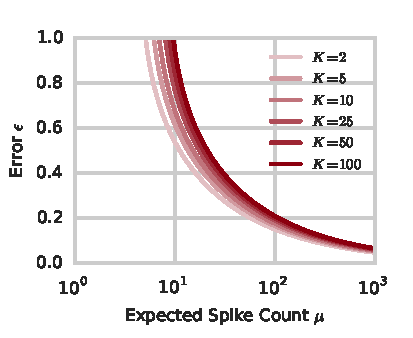
\includegraphics[width=\textwidth]{figures/ch9/error_vs_expected_spike_count}
   \label{fig:error_vs_expected_spike_count}
 \end{subfigure}
 \begin{subfigure}[b]{2.75in}
   \centering
   \caption{}
   \vspace{-.4in}
   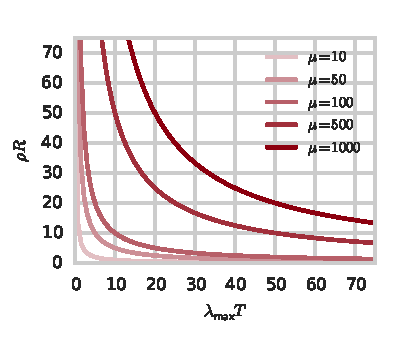
\includegraphics[width=\textwidth]{figures/ch9/mu_for_R_T}
   \label{fig:mu_vs_R_T}
 \end{subfigure}
 \vspace{-.3in}
 \caption[Theoretical bounds on expected spike count and physiological parameters]
 { Theoretical relationship between between $\ell_\infty$-distance, expected spike
   count, and physiological parameters. 
   \textbf{(a)} Theoretical 
   upper bound on the 95th percentile of the $\ell_\infty$-distance,~$\epsilon$, 
   as a function of the expected spike count,~$\mu = (\rho R) (\lambdamax T_I)$,
   for increasing values of~$K$. 
   \textbf{(b)} The expected spike count is the product of the effective number 
   of neurons,~$\rho R$, and the effective number of spikes per neuron,~$\lambdamax T_I$.
   This shows how time and number of neurons can be balanced to obtain the desired 
   expected spike count.
 }
 \label{fig:theoretical_complexity}
\end{figure}

Figure~\ref{fig:theoretical_complexity} plots these theoretical 
bounds. Fig.~\ref{fig:error_vs_expected_spike_count} shows the theoretical
upper bound on the 95th percentile of the $\ell_\infty$-distance as a
function of the expected spike count for a range of distribution sizes,~$K$.
Fig.~\ref{fig:mu_vs_R_T} illustrates the trade-offs between effective 
number of neurons and expected number of spikes per neuron necessary 
to achieve a desired expected spike count.


% Figure: empirical and theoretical $\ell_\infty$-distance
\begin{figure}[t!]
  \centering
  \begin{subfigure}[b]{2.75in}
    \centering
    %\caption{}
    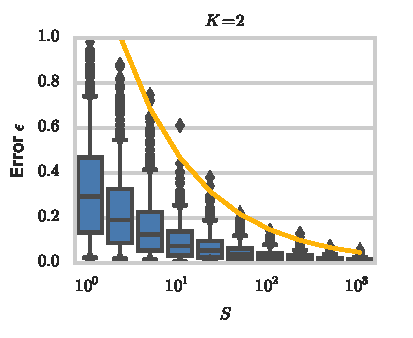
\includegraphics[width=\textwidth]{figures/ch9/error_vs_S_K2}
    \label{fig:error_vs_S_K2}
 \end{subfigure}
 \begin{subfigure}[b]{2.75in}
   \centering
   %\caption{}
   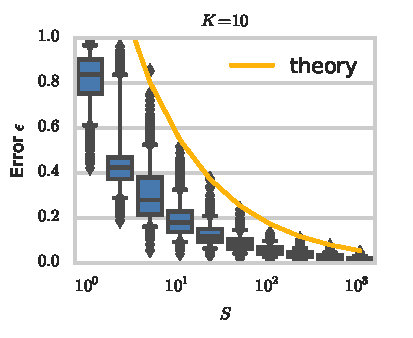
\includegraphics[width=\textwidth]{figures/ch9/error_vs_S_K10}
   \label{fig:error_vs_S_K10}
 \end{subfigure}
 \\
 \vspace{-.25in}
 \begin{subfigure}[b]{2.75in}
   \centering
   %\caption{}
   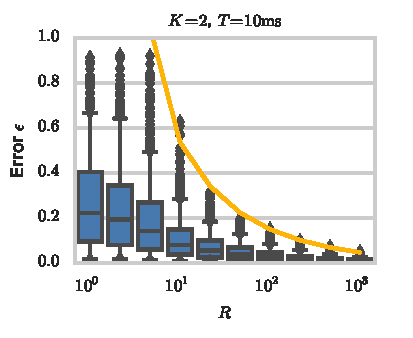
\includegraphics[width=\textwidth]{figures/ch9/error_vs_R_K2}
   \label{fig:error_vs_R_K2}
 \end{subfigure}
 \begin{subfigure}[b]{2.75in}
   \centering
   %\caption{}
   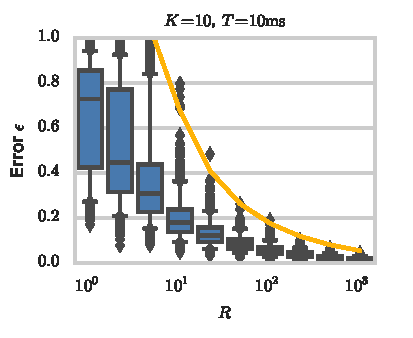
\includegraphics[width=\textwidth]{figures/ch9/error_vs_R_K10}
   \label{fig:error_vs_R_K10}
 \end{subfigure}
 \\
 \vspace{-.25in}
 \begin{subfigure}[b]{2.75in}
   \centering
   %\caption{}
   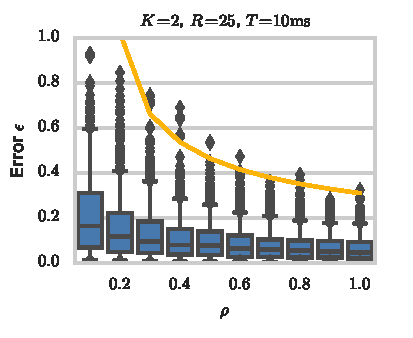
\includegraphics[width=\textwidth]{figures/ch9/error_vs_rho_K2}
   \label{fig:error_vs_rho_K2}
 \end{subfigure}
 \begin{subfigure}[b]{2.75in}
   \centering
   %\caption{}
   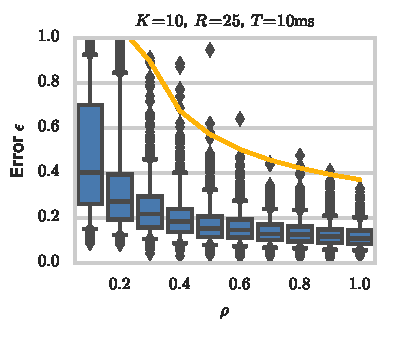
\includegraphics[width=\textwidth]{figures/ch9/error_vs_rho_K10}
   \label{fig:error_vs_rho_K10}
 \end{subfigure}
 \vspace{-.3in}
 \caption[Empirical and theoretical $\ell_\infty$-distance]
 {Empirical and theoretical $\ell_\infty$-distance under a variety 
   of parameter regimes. Whiskers show the empirical~5th 
   and~95th percentiles. Yellow line shows the theoretical
   upper bound on the 95th percentile. 
   \textbf{Left} column:~$K=2$. \textbf{Right} column:~$K=10$. 
   \textbf{Top} row: fixed population spike count,~$S$. 
   \textbf{Middle} row: varying the number of neurons per variable.
   \textbf{Bottom} row: varying the connection probability.
   See text for full description.
 }
 \label{fig:complexity}
\end{figure}

Figure~\ref{fig:complexity} shows the results of an empirical 
assessment of this theory under a variety of parameter regimes.
For each regime, we present results for discrete distributions
over~$K=2$ values (left column) and~$K=10$ values (right column). We 
sample~$1000$ discrete distributions from a Dirichlet 
prior,~${\bpi \sim \distDirichlet(\bone_K)}$, and then we encode each true 
distribution with Poisson spiking neurons and measure the $\ell_\infty$-distance between the true and encoded distributions. 

In the top row, we consider the case where the total population 
spike count is set explicitly, as in Theorem~\ref{thm:fixed_count}.
In this case, the spikes are attributed to each value according 
to a multinomial distribution. We plot the theoretical bound from
Theorem~\ref{thm:fixed_count} in yellow.

In the middle row we measure the error as a function of the
representation size,~$R$, for~$\rho=1.0$, under the assumption that
spikes are counted in one millisecond bins for~$T_I=10$ milliseconds,
and a maximum firing rate of~$100$Hz (i.e.~$\lambdamax=0.1$). Thus, in
expectation the population will emit~$R$ spikes, allowing the top and
middle rows to be directly compared. That is, in the top row, the
population fires exactly the number of spikes expected in the middle
row.  We see that the stochastic population spike counts does indeed
introduce extra variability in the error, as predicted by
Theorem~\ref{thm:rate_bounds}, though the median error is not
substantially different from that of the fixed-$S$ case.

Finally, the bottom row shows the empirical and predicted error as 
we vary the observation probability,~$\rho$. Here, the representation 
size is fixed to~$R=25$, and the gain and integration time are 
set as in the middle row. While a strict upper bound is difficult 
to derive theoretically, the approximation from 
Corollary~\ref{cor:sparse_bounds} provides a reasonable 
approximation for this parameter regime.

These complexity-theoretic bounds relate the number of spikes to the 
distance between the true and estimated distributions.
From the number of spikes, we can deduce constraints on the representation
size, integration time, and connection probability, for realistic gain levels.
While the theoretical bounds do not exactly match the empirical error 
distributions, they appear to be roughly correct up to a multiplicative 
factor. Thus, if we can estimate some biophysical properties like 
connection probabilities, integration times, and firing rates, 
and we can constrain the error 
tolerances of the algorithms that consume these probability estimates, 
then we can estimate the number of neurons that must represent 
each variable-value pair. This will prove useful in guiding our 
bottom-up search, and serve as an important constraint for assessing 
the viability of a direct representation of probability.


% Inference section
\section{Bayesian Inference with Neural Dynamics}
\label{sec:inference}
Two forces cause the encoded distributions to change over time. As
we interact with the world and receive new inputs, the probabilities
of variables change to reflect the new
observations. Moreover, even for a fixed set of observed variable
assignments, the probabilities of latent variables will change as we
perform inference.
%ayesian inference is the process of computing the
%posterior distribution over latent variables given the values of visible inputs.
%Many inference algorithms are iterative, and as they execute,
%the instantaneous probability distribution will change.
We show how a simple, iterative inference algorithm can be
implemented with biologically plausible neural dynamics.

We assume that as an organism receives new inputs from the world, it
updates its posterior distribution over the values of latent
variables. Doing so requires a probabilistic model that relates hidden
and observed variables via a joint probability distribution.  Whereas
in previous chapters we have considered directed graphical models,
here we assume that the probabilistic models implemented in the brain
are best described in terms of a \emph{factor graph},
\begin{align}
  \label{eq:probabilistic_model}
  p(\bz \given \btheta) &=
  \frac{1}{Z(\btheta)}
  \prod_{j \in \mcG} \phi(z_j \given \btheta) \,
  \prod_{i,j \in \mcG} \phi(z_i, z_j \given \btheta) \,
\end{align}
The graph,~$\mcG$, specifies unary and pairwise
probabilistic dependencies between variables.  Each unary factor,~$\phi(\cdot \given
\btheta)$ is a function that maps a variable assignment to a
nonnegative real number, and each pairwise factor,~$\phi(\cdot, \cdot
\given \btheta)$, is a function that maps a pair of assignments,
say~${(z_i=k, z_j=k')}$ to a nonnegative real number. The
normalizing constant,~$Z(\btheta)$, ensures that the joint probability
distribution sums to one.
The probabilistic model in Eq.~\ref{eq:probabilistic_model} reflects
a specific assumption about the types of dependency structures
neural populations can represent.

\begin{assumption}
  Neural populations perform inference in probabilistic models
  that factor into the product of unary and pairwise dependencies. 
\end{assumption}

A general probabilistic model need not factor into pairwise terms. It may instead
have factors that relate three or more latent variables. As we will
see, unary and pairwise factors map naturally onto neural biases
and synaptic weights. In our proposed neural implementation, higher
order factors would require the interaction of three or more neurons.
While this may be realized with dendritic computation or interneurons,
these more sophisticated implementations are beyond the scope of this
chapter. 

In general, the posterior distribution of a subset of hidden
variables~$\bz_H \subseteq \bz$ 
given the observed variables~$\bz_O = \bz \setminus \bz_H$ is,
\begin{align*}
  p(\bz_H \given \bz_O, \btheta) &=
  \frac{p(\bz_H, \bz_O \given \btheta)}
       {\sum_{\bz_H} p(\bz_H, \bz_O \given \btheta)}.
\end{align*}
Typically, this cannot be efficiently computed since it requires a sum
over all possible hidden variable assignments.  However, as we have
seen in previous chapters, there are many methods of approximating
posterior distributions. Mean field variational inference maps
particularly nicely onto the natural constraints of neural dynamics.
In mean field variational inference, the intractable exact
posterior distribution is approximated with a tractable, factorized distribution,
\begin{align*}
  p(\bz_H \given \bz_O, \btheta) &\approx q(\bz_H) \equiv \prod_{z_j \in \bz_H} q(z_j).
\end{align*}
The terms in this product are called \emph{variational factors}.  We
solve for the variational factors that minimize KL-divergence between
the true and approximate posterior,~$\KL(q(\bz_H) \,||\, p(\bz_H
\given \bz_O, \btheta))$. In minimizing the KL-divergence, we
simultaneously maximize a lower bound on the log marginal
likelihood,~$\log p(\bz_O \given \btheta)$.

The simplest method of minimizing this objective is via coordinate
descent, iteratively updating the probability of one hidden variable
given the probabilities of the rest. Since our variational
distribution is factorized, the variational factor for variable~$z_j$
must satisfy the mean field consistency equation:
\begin{align}
  \label{eq:mf_consistency}
  \log q(z_j) &\simeq \bbE_{q(\bz_{\neg j})}
  \left[ \log p(\bz_H, \bz_O \given \btheta) \right],
\end{align}
where~$\simeq$ denotes equality up to an additive constant and the
expectations are taken with respect to the variational
distribution over other hidden variables,
\begin{align*}
  q(\bz_{\neg j}) &= \prod_{i \neq j} q(z_{i}).
\end{align*}
The additive constant
ensures normalization of the probabilities, and will be discussed
subsequently.  

For discrete random variables, the variational factors are simply
vectors specifying the posterior probability of each variable,~$z_j$.
Under the direct representation described above, the instantaneous
values of these factors are encoded in the relative spike counts of
populations of neurons,
\begin{align*}
  q_t(z_j=k) &= \widehat{\pi}_{t,k}^{(j)} 
\end{align*}
To perform inference, the neuronal dynamics must be such that at each
time step, the relative spike counts satisfy~Eq.~\ref{eq:mf_consistency}. 
%For discrete random variables, this implies that the rate of a neuron~$n$
%that represents the variable-value pair~(${j_n=j,\,k_n=k}$) should obey,
Explicitly writing the additive constant,~$-\log \nu_t^{(j)}$, we have,
\begin{align}
  \nonumber
  \log \widehat{\pi}_{t,k}^{(j)} 
  &= -\log \nu_t^{(j)} + \log \phi(z_j=k \given \btheta) \\
  \nonumber
  &\hspace{4em} + \bbE_{q_{t-1}(\bz_{\neg j})} \bigg[
  \sum_{i \in \neigh(j)} \log \phi(z_{i}, z_j=k \given \btheta) \bigg] \\
  % In terms of firing rates
  & \nonumber = 
     - \log \nu_t^{(j)} + \log \phi(z_j=k \given \btheta) \\
  &   \label{eq:variational_rate}
  \hspace{4em} + \sum_{i \in \neigh(j)} \sum_{k'=1}^K
  \bigg[\log \phi(z_{i}=k', z_j=k \given \btheta) \,\cdot  \widehat{\pi}_{t-1,k'}^{(i)} \bigg] \\
  \nonumber
  &= -\log \nu_t^{(j)} + \psi_{t,k}^{(j)},
\end{align}
where
\begin{align*}
  \psi_{t,k}^{(j)} &=
  \log \phi(z_j=k \given \btheta)
  + \sum_{i \in \neigh(j)} \sum_{k'=1}^K
  \log \phi(z_{i}=k', z_j=k \given \btheta) \,\cdot  \widehat{\pi}_{t-1,k'}^{(i)}.
\end{align*}
%where we have combined the terms from the unary and pairwise factors
%into the activation,~$\psi_{t,k}^{(j)}$.

Since~$\widehat{\bpi}_{t}^{(j)}$ is a probability distribution, 
 the additive constant must be set to it is normalized.  Thus,
\begin{align*}
  \widehat{\pi}_{t,k}^{(j)} &=
  \exp \left \{\psi_{t,k}^{(j)} -\log \nu_{t}^{(j)} \right \} \\
  \implies
  \nu_t^{(j)} &= \sum_{k'} \exp \left \{\psi_{t,k'}^{(j)} \right \}.
\end{align*}

%Note that the pairwise factor functions are not necessarily symmetric.
%In fact, the two variables may have support for different ranges of
%values, so symmetry often does not make sense.  We have written this
%such that~$z_j$ is always the second argument, but its order will
%depend on its role in each factor.

Now that we have derived theoretically exact mean field updates, we
must show how they can be approximated with plausible neural dynamics.
We assume that inference occurs on a characteristic time scale of~$T_I$
time steps. This reflects the window of time over which neurons estimate
probability distributions.
From Lemma~\ref{lem:consistency}, we know that if the firing rates of
neurons the variable-value pair~${(z_j,k)}$ are proportional
to~$\widehat{\pi}_{t,k}^{(j)}$, then in expectation, the empirical
distribution represented by the spike counts will be equal to the
desired distribution. Thus, we aim to set,
\begin{align*}
  \lambda_{t,n} &= \lambdamax \, \widehat{\pi}_{t,k_n}^{(j_n)}
  = \lambdamax \exp \left \{\psi_{t,k_n}^{(j_n)} -\log \nu_{t}^{(j_n)} \right \},
\end{align*}
for maximum firing rate,~$\lambdamax$. While this rate function is
nearly a linear-nonlinear cascade, as we studied in previous
chapters, there is one major impediment to realizing this
calculation in biological neurons. Specifically, to compute
the activation, a neuron must have access to the \emph{normalized}
probabilities of other hidden and visible variables. In practice,
a neuron only observes the spike counts of the neurons it receives 
input from. However, these can be used to estimate the desired probabilities.
This motivates our next assumptions,

\begin{assumption}
  Neurons are sparsely connected to one another. For each ordered
  pair of neurons, $(m,n)$, the variable~$a_{m \to n} \in \{0,1\}$
  indicates whether or not there exists a synaptic connection from
  neuron~$m$ to neuron~$n$. These connections are modeled as
  independent and identically distributed Bernoulli random variables,
  \begin{align*}
    a_{m \to n} &\sim \distBernoulli(\rho).
  \end{align*}
  We combine these variables into a binary adjacency 
  matrix,~$\bA \in \{0,1\}^{N \times N}$.
\end{assumption}

\begin{assumption}
  All neurons in the population share the same gain,~$\lambdamax$. 
  Thus, neuron~$n$'s estimate of~$\bpi^{(j)}$ is 
  informed by~$(\lambdamax T_I)(\rho R)$ spikes, in expectation:
  \begin{align*}
    \bbE_{\bA,\bs} \bigg[ \sum_{\Delta = 1}^{T_I} & \sum_{m=1}^N \bbI[j_m=j] \, a_{m \to n} \cdot s_{t-\Delta,m} \bigg] \\
    &= \bbE_{\bA,\bs} \left[ \sum_{\Delta = 1}^{T_I} \sum_{m=1}^N \sum_{k=1}^K \bbI[j_m=j, k_m=k] \, a_{m \to n} \cdot s_{t,m} \right] \\
    &= \lambdamax T_I \rho \sum_{m=1}^N \sum_{k=1}^K \bbI[j_m=j, k_m=k] \, \widehat{\pi}_{t,k}^{(j)} \\
    &= (\lambdamax T_I) (\rho R).
  \end{align*}

  Moreover, the instantaneous probability is well-approximated by,
  \begin{align*}
      \widehat{\pi}_{t,k}^{(j)} &=
  \frac{\sum_{\Delta=1}^{T_I} \sum_{m=1}^N \bbI[j_m=j, k_m=k] \, a_{m \to n} \cdot s_{t-\Delta, m}}
       {\sum_{\Delta=1}^{T_I} \sum_{m=1}^N \bbI[j_m=j] \, a_{m \to n} \cdot s_{t-\Delta, m}} \\
       &\approx (\lambdamax T_I \rho R)^{-1} \sum_{\Delta=1}^{T_I} \sum_{m=1}^N \bbI[j_m=j, k_m=k] \, a_{m \to n} \cdot s_{t-\Delta, m}.
  \end{align*}
  In other words, the total spike count is concentrated around its mean.
\end{assumption}

Under the assumption of shared gain, the
desired dynamics in~Eq.~\ref{eq:variational_rate}
simplify to,
\begin{align}
  \label{eq:mf_log_probs}
  \lambda_{t,n} &= \lambdamax
  \exp \left \{b_n + (\lambdamax T_I \rho R)^{-1} \sum_{\Delta=1}^{T_I} \sum_{m=1}^N a_{m \to n} \cdot w_{m \to n} \cdot s_{t-\Delta,m}
  - \log \nu_t^{(j_n)} \right \}
\end{align}
where
\begin{align*}
  b_n &= \log \phi(z_{j_n} = k_n \given \btheta),
\end{align*}
and
\begin{align*}
  w_{m \to n} &=
  \begin{cases}
    \log \phi(z_{j_n}=k_n, z_{j_m}=k_m \given \btheta) & \text{if }j_m
    \in \neigh(j_n) \\
    0 & \text{o.w.}
  \end{cases}
\end{align*}
Thus, the theory provides a normative interpretation of synaptic
weights: they reflect the conditional log probabilities for the
variable-value pairs represented by the pre- and post-synaptic
neurons.


The last step is to compute the normalizing input,~$\nu_t^{(j)}$.
This requires summing the instantaneous rates of all neurons representing the
random variable,~$z_j$. While this is clearly implausible, we may derive
a gain controller from an alternative perspective. Normalizing the
probability distribution ensures that the expected spike count at
any time step for
neurons representing~$z_j$ is equal to~$\lambdamax R$. If the distribution
is not properly normalized, the expected spike count will deviate.
Thus, a reasonable gain controller can estimate the population
can estimate the population rate,
\begin{align*}
\widehat{\lambda}_{t}^{(j)} &= \sum_{\Delta = 1}^{T_G} \sum_{n=1}^N \bbI[j_n=j] s_{t-\Delta, n},
\end{align*}
and set the control input to,
\begin{align*}
  \nu_{t}^{(j)} &= \frac{\widehat{\lambda}_{t}^{(j)}}{\lambdamax T_G R}.
\end{align*}
The time scale of the gain controller is typically
less than the time scale of inference, that is~$T_G < T_I$.

Having shown that variational inference is theoretically plausible,
we consider a simple example.

\section{Example of a Simple Mixture Model}
\label{sec:mixture_example}

% Figure: Example of neural inference in a simple mixture model
\begin{figure}[t!]
  \centering
  \begin{subfigure}[b]{5.5in}
   \centering
   \caption{}
   \vspace{-.3in}
   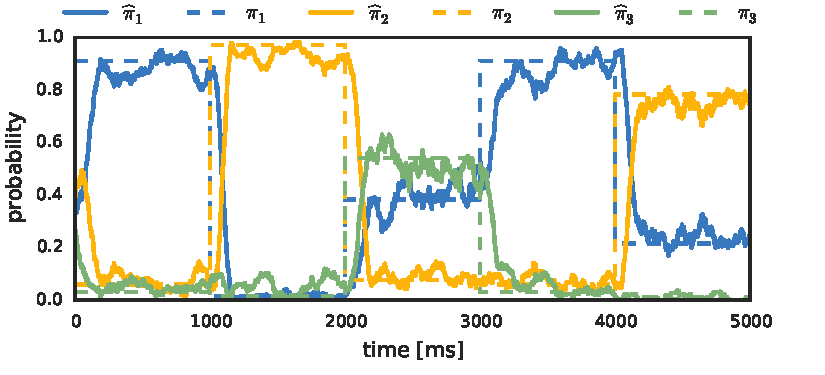
\includegraphics[width=\textwidth]{figures/ch9/neural_mixture_probs}
   \label{fig:mixture_probs}
 \end{subfigure} \\
 \begin{subfigure}[b]{5.5in}
   \centering
   \caption{}
   \vspace{-.4in}
   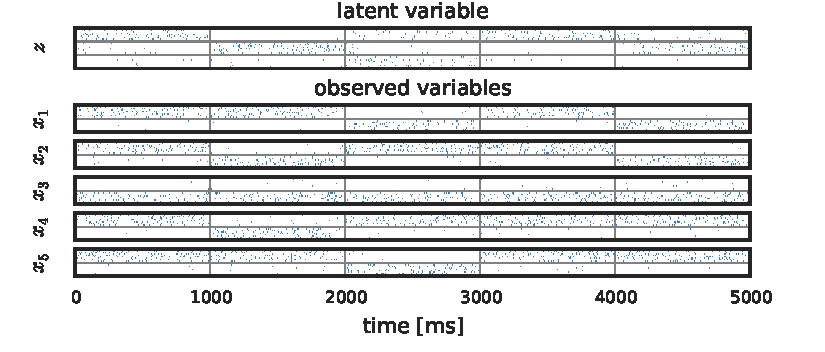
\includegraphics[width=\textwidth]{figures/ch9/neural_mixture_spiketrains}
   \label{fig:mixture_spiketrains}
 \end{subfigure}
 \vspace{-.3in}
 \caption[Demo of neural inference in a simple mixture model]
         {Example of neural inference  a simple mixture model with one
           latent variable,~$z \in \{1, 2, 3\}$, indicating which of the
           three mixture components gave rise to the data. The observations
           consist of 5 conditionally independent binary
           variables,~$x_1, \ldots, x_5$, whose values change every second. 
           %Each variable-value pair is represented by~$R=10$ neurons.
           \textbf{(a)} The empirical probabilities (solid lines) decoded
           from the spike train, and the true posterior (dashed line).
           Stochasticity arises from noisy inputs and Poisson spike counts.
           \textbf{(b)} The underlying spike trains of the neurons representing
           ~$z$ and~$x_i$. Horizontal gray lines distinguish subpopulations of~$R=10$ neurons for
           each value; vertical lines denote times of stimulus change.
 }
 \label{fig:mixture}
\end{figure}


Consider a simple mixture model with a single
latent variable denoting the mixture component,~${z \in \{1, \ldots, K\}}$,
and a set of conditionally independent observations,~$\{x_j\}_{j=1}^J$.
In this example, we let the observations be Bernoulli
random variables. The model is parameterized by a marginal
class probability vector,~$\balpha$, which we assume is uniform,
and class-conditional probabilities for each observation,
${p_{j,k} = \Pr(x_j=1 \given z=k)}$. Together, these
specify the probabilistic model,
\begin{align*}
  \balpha &= \tfrac{1}{K} \bone, & & &
  z &\sim \distDiscrete(\balpha), \\
  p_{j,k} &\sim \distBeta(\tfrac{1}{2},\tfrac{1}{2}),  & & &
  x_j &\sim \distBernoulli(p_{j,z}).  
\end{align*}
This corresponds to a factor graph with,
\begin{align*}
  \phi(z=k) &= \alpha_k, \\
  \phi(x_j=1, z=k) &= p_{j,k}, \\
  \phi(x_j=0, z=k) &= 1-p_{j,k}.
\end{align*}

We simulate inference in this model with a population of neurons.
Each variable-value pair is represented by~$R=10$ neurons, and each
pair of neurons is connected with probability~$\rho=0.5$. The maximum
firing rate is set to~$\lambdamax=100\text{Hz}$, and the integration
time window is set to~$T_I=100\text{ms}$. Hence, the expected spike
count used to estimate probabilities is~$(\rho R)(\lambdamax T_I)
= 50$ spikes. The neurons representing the observed variable assignment
~$x_j=k$ are externally driven at a rate of~$0.95 \lambdamax$ if~$x_j=k$,
and a rate of~$0.05 \lambdamax$ if~$x_j \neq k$. We assume that the
synaptic weights have already been learned and reflect the exact
log of the pairwise factors. 

Figure~\ref{fig:mixture} illustrates inference dynamics for a
changing stimulus. Every second, the observed variables are driven with
a new pattern, which leads to a new posterior distribution over the
latent variable. With each change in input, the neurons representing the
latent variable adjust their firing rates to reflect this new probability.
Fig.~\ref{fig:mixture_probs} shows the decoded probabilities over time
(solid lines) along with the true posterior (dashed lines). Despite many
sources of stochasticity, the decoded probabilities do converge to
the correct posterior values. The $100$ms integration time is reflected in
the delayed convergence upon each change in stimulus.
Fig.~\ref{fig:mixture_spiketrains} shows the spike trains from which these
probabilities were decoded. The neurons are ordered according to
the value they encode and the subpopulations of~$R$ neurons are
separated by horizontal light gray lines. Vertical lines indicate changes
in input. Overall, the neurons fire at between $30$ and $40$Hz, with a
dynamic range of about $0$ to $100$Hz, as expected.



\section{Reverse Engineering the Probabilistic Model from Spike Trains}
\label{sec:reverse_engineering}

Given this ``top-down'' theory of neural computation, can we reverse
engineer the probabilistic model from neural recordings? To do so, we
need to infer the subpopulations of neurons that encode each
variable-value pair, as well as the characteristic weights that
connect each subpopulation.  We show that this is possible using the
generalized linear models and structured network priors described in
Chapter~\ref{chap:five}.

Recall the theoretical dynamics proposed in Section~\ref{sec:inference},
 reproduced here in slightly simplified form,
\begin{align*}
  \lambda_{t,n} &= \lambdamax
  \exp \left \{b_n + \gamma \sum_{\Delta=1}^{T_I} \sum_{m=1}^N a_{m \to n} \cdot w_{m \to n} \cdot s_{t-\Delta,m}
  - \log \nu_t^{(j_n)} \right \}.
\end{align*}
The instantaneous firing rate take the form of a generalized linear model.
Each neuron has a baseline rate that is a function of~$b_n$ and~$\lambdamax$.
Moreover, the rate is influenced by recent spiking activity through
the network,~$\bA \odot \bW$, and through the local normalization,~$\nu$. 

According to our theory of neural inference, the sparsity pattern of
the network should follow an independent Bernoulli model. That is,
each edge is present with the same probability,~${a_{m \to n} \sim
  \distBernoulli(\rho)}$.  Moreover, the weights of network should
encode the pairwise log probabilities,~${\log \phi(z_i=k, z_j=k')}$,
and the weights from the~$R$ neurons representing~${z_i=k}$ to the~$R$
neurons representing~${z_j=k'}$ should all be approximately
equal. This corresponds to stochastic block structure in the weight
matrix. Thus, to reverse engineer the probabilistic model from the
observed spike train, we fit a generalized linear model with a
spike-and-slab network prior that has an independent Bernoulli model
for the adjacency matrix, and a stochastic block model (SBM) for the
weight matrix. The SBM has latent variables for each neuron that
indicate the cluster assignment, and parameters that specify the
average weight between each pair of clusters:
\begin{align*}
  c_n & \sim \distDiscrete(\alpha \bone), \\
  \mu_{c \to c'} &\sim \distGaussian(0, \sigma_0^2), \\
  w_{m \to n} &\sim \distGaussian(\mu_{c_m \to c_n}, \sigma^2).
\end{align*}
By performing Bayesian inference in this model, we recover a posterior
distribution over biases,~$\{b_n\}_{n=1}^N$; weighted adjacency
matrices,~$\bA$ and~$\bW$; latent variables,~$\{c_n\}_{n=1}^N$; and
parameters,~$\{\mu_{c \to c'}\}_{c,c'=1}^C$.

The normalization presents a minor complication. According to the
theory, this is most likely computed by local inhibitory neurons
that estimate the population rate of neurons representing~$z_j$
and deliver a common, normalizing input to stabilize the rate
at the desired level. This can be roughly approximated with
direct, excitatory connections between neurons representing the same
variable-value pair, and inhibitory connections between neurons
representing competing values of the same variable. In other words,
if we focus solely on the activity of neurons representing the variable-value
pairs, we should expect additional \emph{functional} connections
that encode the mutually exclusive nature of the distinct values
of a given variable.

% Figure: Example of neural inference in a simple mixture model
\begin{figure}[t!]
  \centering
  \begin{subfigure}[b]{2.75in}
   \centering
   \caption{}
   \vspace{-.3in}
   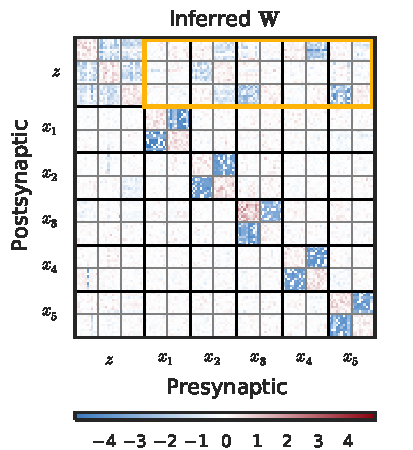
\includegraphics[width=\textwidth]{figures/ch9/mixture_network}
   \label{fig:mixture_network}
  \end{subfigure}
  ~
  \begin{subfigure}[b]{2.75in}
   \centering
   \caption{}
   \vspace{-.3in}
   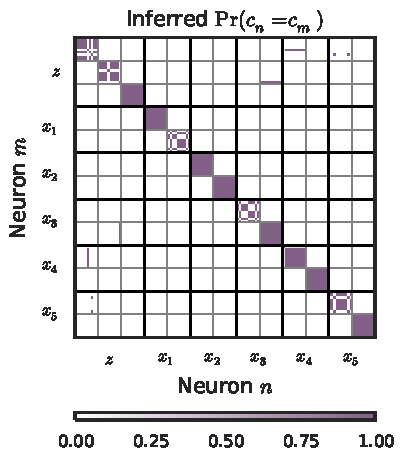
\includegraphics[width=\textwidth]{figures/ch9/mixture_cocluster_probability}
   \label{fig:mixture_cocluster}
 \end{subfigure} \\
 \begin{subfigure}[b]{5.5in}
   \centering
   \caption{}
   \vspace{-.4in}
   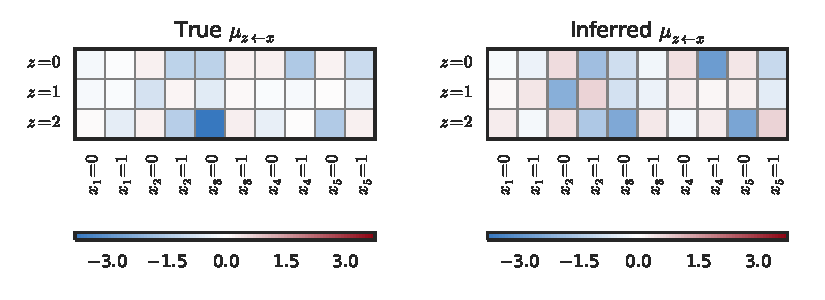
\includegraphics[width=\textwidth]{figures/ch9/mixture_prob_weights}
   \label{fig:mixture_prob_weights}
 \end{subfigure}
 \vspace{-.3in}
 \caption[Reverse engineering probabilistic models from neural spike
   trains] {The probabilistic model can be reverse engineered from the
   neural spike train.
   \textbf{(a)} Inferred weighted adjacency matrix for the population
   of $130$ neurons. Thin lines delineate boundaries between subpopulations
   for each value of~$z$ and~$x_j$; bold lines separate populations for
   each variable. 
   \textbf{(b)} Inferred probability that each pair of neurons belongs to
   the same cluster under a stochastic block model.
   The block diagonal structure shows that the
   variable-value subpopulations are clearly recovered.
   \textbf{(c)} True and inferred weights
   from~$x_j$ to~$z$ (yellow square in~\textbf{(a)}). Inferred weights
   are the mean weights under the stochastic block model. They accurately
   recover the true weights.
 }
 \label{fig:mixture_recovery}
\end{figure}

We demonstrate this approach by fitting the hierarchical model to a
neural spike train simulated from the population described in
Section~\ref{sec:mixture_example}. The population performs inference
in a simple mixture model with three latent mixture components, and
five binary observations. An observation consists of an assignment of
the five observations, indicated by the variables~$\{x_j\}_{j=1}^5$,
and given an observation, the dynamics perform posterior inference
of~$z$, the latent variable indicating the underlying mixture
component. The population consists of $130$ neurons, $10$ for each
variable-value pair.



Figure~\ref{fig:mixture_recovery} shows the inferred parameters of the
hierarchical model. The posterior mean of the weighted adjacency
matrix is shown in Figure~\ref{fig:mixture_network}, with neurons sorted
by variable and then by value. The block diagonal structure shows
the normalizing connections between neurons representing the same variable,
and the region highlighted in yellow shows the inferred connections from
neurons representing~$x_j$ to neurons representing~$z$. These encode
the pairwise log probabilities of the mixture model.

Figure~\ref{fig:mixture_cocluster} shows the inferred posterior probability
of two neurons belonging to the same cluster. While the true model has
$13$ clusters, we allowed our model to use as many as $20$ clusters.
If the variable-value subpopulations
were recovered perfectly, this matrix would be block diagonal. We
see that it is nearly so; only a handful of neurons are misclassified
and some blocks are split in two.

Finally, Figure~\ref{fig:mixture_prob_weights} shows the true and inferred
mean weights under the stochastic block model. First, we found the permutation
of inferred cluster labels that best matched the true cluster labels. Then we found the
linear transformation that best matched the true and inferred weights.
The result shows that the true pattern of weights from~$x_j$ to~$z$ are
recovered with high fidelity.

While this procedure for reverse engineering probabilistic models
from observed spike trains is not foolproof, this simple example
illustrates that much can be learned by combining top-down theories
with bottom-up analysis. To further improve this inference procedure,
we should include two sets of latent cluster assignments in our
hierarchical model: one set of variables that specifies the
variable that a cluster of neurons represents (i.e.~$j_n$ in our
theory), and another that indicates the value (i.e.~$k_n$).
Incorporating the knowledge that different values of the same variable
are mutually exclusive, we can build a strong prior distribution
over weights given these two variables. 

What else can be learned from the results of this approach? In
practice, we only observe a fraction of the neurons in a particular
region If our recording method samples~$N$ neurons out
of~$N_{\mathsf{total}}$, then given an inferred block
size,~$\widehat{R}$, we can estimate the true representation size to
be roughly,~$R\approx \widehat{R} N_{\mathsf{total}} / N$. If variable-value
subpopulations are truly disjoint, this provides an estimate of the
number of subpopulations the region could encode. Combined with the
complexity theoretic bounds developed in Section~\ref{sec:complexity},
these top-down and bottom-up approaches provide two tacks  by which we may 
converge on a theory of probabilistic inference in neural circuits.

\section{Future Work}
\label{sec:future}

This chapter has illustrated how theoretical models of neural computation
may be assessed from a ``top-down'' perspective by analyzing the complexity
and comparing it to biological parameters, and from the ``bottom-up'' perspective,
by incorporating theoretical dynamics into probabilistic models of neural
population activity. This is only a first step toward closing the gap
between these two perspectives, and it opens many important questions.
We enumerate and partially answer a few of them here.

\subsection{Unsupervised Learning via Synaptic Plasticity}
\label{sec:learning}
Perhaps the most pressing question is that of learning: how are these
subpopulations of neurons and their weighted connections established?
While we do not have a concrete answer to this question, we
speculate that subpopulations are primarily allocated in a supervised
fashion by a process like those of~\citet{valiant1994circuits}.
Once the neurons have been allocated, their weights may be tuned
in an unsupervised manner. We suggest one way in which this unsupervised
learning may be related to the process of spike-timing dependent
plasticity, based on the work of \citet{nessler2013bayesian}.

The parameters of the model,~$\btheta$, specify the conditional
probabilities for pairs of hidden and visible variables. Rather than
treating the parameters as given, we now treat them as part of the
model.
\begin{align*}
  p(\bz, \btheta) &= p(\btheta) \, p(\bz \given \btheta)  \\
  &= \frac{p(\btheta)}{Z(\btheta)} \prod_{j \in \mcG} \phi(z_j \given \btheta)
  \prod_{i,j \in \mcG} \phi(z_i, z_{j} \given \btheta).
\end{align*}
The challenge with learning is that the parameters appear in the
normalizing constant,~$Z(\btheta)$, which is typically an intractable
summation over variable assignments. For this simple example,
we will only consider learning in a subset of models that can
formulated as directed graphical models.

\begin{assumption}
  The following unsupervised learning algorithm assumes that the probabilistic
  model not only factors into the product of unary and pairwise
  potentials, but that this factorization corresponds to a directed
  graphical model in which the variables have at most one ``parent''
  variable. That is, the variables are ordered such that the
  joint probability is equal to,
  \begin{align*}
    p(\bz, \btheta) &= p(\btheta) \prod_{j=1}^J p(z_j \given \pa(z_j), \btheta),
  \end{align*}
  where~$\pa(z_j) \in \{\varnothing, z_1, \ldots, z_{j-1}\}$.
  Each conditional distribution in this product is properly normalized,
  which implies that the joint distribution is normalized as well.
\end{assumption}

While this is clearly a strict assumption, it allows
for some realistic models like mixtures and hidden Markov models.
The advantage is that, here, the
distribution is normalized such that the parameters appear only
in their prior and in the conditional distributions, which depend
on at most two variables. This will map nicely onto synaptic plasticity
rules. 

Since we are assuming the variables
are discrete, the parameters~$\btheta$ specify either the marginal
probability of~$z_j$ (if~$\pa(z_j)=\varnothing$) or the rows of a
conditional probability table (if~${\pa(z_j) \in \{z_1, \ldots, z_{j-1}\}}$).
We
make this explicit with the following notation,
\begin{align*}
  p(z_j \given \pa(z_j)=\varnothing, \btheta) &= \distDiscrete(\btheta^{(j)}), \\
  p(z_j \given \pa(z_{j})=z_{j'}=k, \btheta) &=  \distDiscrete(\btheta^{(j,k)}).
\end{align*}
In words, if the variable~$z_j$ has no parent, it is marginally distributed
according to a categorical distribution with parameter~$\btheta^{(j)}$.
If variable~$z_j$ has parent~$z_{j'}$, then when~$z_{j'}=k$, the
variable~$z_j$ follows a categorical distribution with
parameter~$\btheta^{(j,k)}$. 

To incorporate these parameters into the model, we introduce Dirichlet priors
over the probability vectors,
\begin{align*}
  \btheta^{(j)} &\sim \distDirichlet(\alpha \bone), & & &
  \btheta^{(j,k)} &\sim \distDirichlet(\alpha \bone).
\end{align*}

Learning in a Bayesian framework corresponds to performing posterior
inference over the parameters. Thus, we introduce a variational factor
for~$\btheta$ as well,
\begin{align*}
  q(\btheta) &=
  \prod_{j: \pa(z_j)=\varnothing} q(\btheta^{(j)})
  \prod_{j: \pa(z_j)\neq \varnothing} \prod_{k} q(\btheta^{(j,k)})
\end{align*}
%Now consider the mean field consistency equation governing the parameter
%of a root variable (with no parent),
%\begin{align*}
%  \log q_t(\btheta^{(j)}) &\simeq
%  \bbE_{q_{t-1}(\bz)}\left[ \log p(\bz, \btheta) \right] \\
%  &\simeq \bbE_{q_{t-1}(\bz)}
%  \left[ \sum_{k=1}^K \bbI[z_j=k] \log \theta_k^{(j)} \right]
%  + \sum_{k=1}^K (\alpha-1) \log \theta_k^{(j)}  \\
%  &\simeq  \sum_{k=1}^K (\widehat{\pi}_{t-1,k}^{(j)} + \alpha-1) \log \theta_k^{(j)}
%\end{align*}
%This is the form of a Dirichlet distribution, which implies,
%\begin{align*}
%  q_t(\btheta^{(j)})
%  &= \distDirichlet(\btheta^{(j)} \given  \balpha_{t}^{(j)}) \\
%  \balpha_{t}^{(j)} &= \alpha + \widehat{\bpi}_{t-1}^{(j)}
%\end{align*}
Consider the variational factor for~$\btheta^{(j,k)}$.  Omitting the
details, we can show that this factor takes the form of a Dirichlet
distribution,
\begin{align*}
  q_t(\btheta^{(j,k)}) &=
  \distDirichlet(\btheta^{(j,k)} \given \balpha_{t}^{(j,k)}), \\
  \balpha_{t}^{(j,k)} &= \alpha + \widehat{\bpi}_{t-1}^{(j)} \cdot \widehat{\pi}_{t-1,k}^{(\pa(z_j))}.
  %q_t(\theta_{k,k'}^{(v,h)}) &=
  %\distGamma(\theta_{k,k'}^{(v,h)} \given
  %\alpha + \widehat{\pi}_{t-1,k}^{(v)} \cdot \widehat{\pi}_{t-1,k'}^{(j)},
  %\, \beta).
\end{align*}
The updates of~$q(z_j)$ must consider expectations with respect to
this Dirichlet factor:
%Returning to the task of inferring the posterior distribution over
%hidden variables, we see that the updates for~$q(z_j)$ must now
%be derived with respect to the expectation of~$q(\btheta)$ as well,
\begin{align*}
  \log q(z_j) &\simeq \bbE_{q(\bz_{\neg j})} \bbE_{q(\btheta)} \left[ p(\bz, \btheta) \right].
\end{align*}
%Instead of working directly with~$\log p(z_j \given \pa(z_j), \btheta)$,
%the updates must work with its expectation under the Dirichlet
%variational factor. If~$\pa(z_j)=\varnothing$, we have
%\begin{align}
%  \nonumber
%  \bbE_{q_t(\btheta)} \left[\log p(z_j=k \given \pa(z_j)=\varnothing, \btheta)\right]
%  &= \bbE_{q_t(\btheta)} \left[\log \theta_{k}^{(j)} \right] \\
%  \nonumber
%  &= \psi\big(\alpha_{t,k}^{(j)}\big)
%  - \psi\big(\sum_{i=1}^K \alpha_{t,i}^{(j)} \big) \\
%  \nonumber
%  &= \psi\big(\alpha_{t,k}^{(j)}\big)
%  - \psi\big(\sum_{i=1}^K \alpha + \widehat{\pi}_{t-1,i}^{(j)} \big) \\
%  \label{eq:expected_log_theta}
%  &= \psi\big(\alpha_{t,k}^{(j)}\big)
%  - \psi\big(K\alpha\big).
%\end{align}
%where~$\psi(\cdot)$ is the digamma function.
This expecation is given by,
\begin{align}
  \nonumber
  \bbE_{q_t(\btheta)} \left[\log p(z_j=k \given \pa(z_j)=k', \btheta)\right]
  &= \bbE_{q_t(\btheta)} \left[\log \theta_{k}^{(j,k')} \right] \\
  \nonumber
  &= \psi\big(\alpha_{t,k}^{(j,k')}\big)
  - \psi\big(\sum_{i=1}^K \alpha_{t,i}^{(j,k')} \big) \\
%  \nonumber
%  &= \psi\big(\alpha_{t,k}^{(j,k')}\big)
%  - \psi\big(\sum_{i=1}^K \alpha + \widehat{\pi}_{t-1,i}^{(j)} \widehat{\pi}_{t-1,k'}^{(\pa(z_j)} \big) \\
  \label{eq:expected_log_theta_syn}
  &= \psi\big(\alpha_{t,k}^{(j,k')}\big)
  - \psi\big(K\alpha + \widehat{\pi}_{t-1,k'}^{(\pa(z_j)} \big).
\end{align}

How could this be implemented biologically?
First, we assume that learning occurs on a 
timescale of~$T_L$ time steps, which is relatively slow compared to
the time scales of inference and behavior. That is,~$T_I < T_L$.
This allows the learning algorithm to generalize from many
input rather than overfitting to a single example.

%For root variables,~$\theta_k^{(j)}$ sets an activation bias that sets
%the baseline firing rate. We assume that these neurons have a dynamic
%state variable,~$\alpha_{t,n}$, that roughly computes a moving average
%of its firing rate,
%\begin{align*}
%  \alpha_{t,n} &= \alpha + (\lambdamax T_L)^{-1} \cdot \sum_{\Delta = 1}^{T_L} s_{t-\Delta ,n} \\
%  &\approx \alpha + \widehat{\pi}_{t,k_n}^{(j_n)}
%\end{align*}
%This state variable governs the instantaneous activation bias,
%\begin{align*}
%  b_{t,n} &= \psi \big(\alpha_{t,n} \big) - \psi \big( K\alpha \big).
%\end{align*}
%If a neuron tends to have a high firing rate, reflecting a high 
%marginal posterior probability, this will eventually be learned and
%incorporated into the activation bias.


We want the synaptic weights to equal the expected log parameter
value, as in~\eqref{eq:expected_log_theta_syn}.  In theory, the weights
should be identical for all synapses between neurons
representing~${(z_j=k)}$ and neurons representing~${(z_{j'}=k')}$.  It is
unreasonable to assume this in practice, since these synapses exist between
different neurons and are updated independently. However, we can
specify a simple learning rule that would give rise to the same
weights in expectation.

Assume that each synapse has a two latent state
variabless,~$\alpha_{t, m \to n}$, and~$\beta_{t,m \to n}$. These will
enable us to compute the expectation with respect to the variational
parameter.  We propose the following learning rule for the first
state,
\begin{align*}
  \alpha_{t, m \to n} &=
  \alpha +
  (\lambdamax^2 T_L)^{-1}  \sum_{\Delta = 1}^{T_L} s_{t-\Delta ,n} \cdot s_{t-\Delta,m} \\
  &\approx \alpha + \widehat{\pi}_{t-1,k_n}^{(j_n)} \cdot \widehat{\pi}_{t-1,k_m}^{(j_m)}. 
\end{align*}
%The tricky, asymmetric part comes in whether the is on the
%child neuron,~$z_{j_m} = \pa(z_{j_n})$, or the parent
%neuron,~$z_{j_n}= \pa(z_{j_m})$. This determines how the second
%state must be computed. If~$z_{j_n}$ is the child, then
Suppose neuron~$n$ represents the child variable and neuron~$m$
represents the parent variable. Then,\footnote{Here, the synaptic state
  variable counts spikes on the pre-synaptic neuron.  If the
  parent-child order was flipped, the synapse would have to count
  post-synaptic spikes instead. This asymmetry is admittedly somewhat
  unsatisfying.  }
\begin{align*}
  \beta_{t,m \to n} &= K\alpha + (\lambdamax T_L)^{-1} \sum_{\Delta = 1}^{T_L} s_{t -\Delta, m} \\
  &\approx K\alpha + \widehat{\pi}_{t-1,k_m}^{(z_{j_m})}.
\end{align*}
%Otherwise, if~$z_{j_n} = \pa(z_{j_m})$,
%\begin{align*}
%  \beta_{t,m \to n} &= K\alpha + (\lambdamax T_L)^{-1} \sum_{\Delta = 1}^{T_L} s_{t -\Delta, n} \\
%  &\approx K\alpha + \widehat{\pi}_{t-1,k_n}^{(z_{j_n})}.
%\end{align*}
%The difference is in whether the second state counts pre- or post-synaptic
%spikes. 
The synaptic weight is then a deterministic function of these two state variables,
\begin{align*}
  w_{t, m \to n} &= \psi(\alpha_{t, m \to n}) - \psi(\beta_{t, m \to n}).
\end{align*}
This state-based learning rule is Hebbian in that correlated spiking
activity leads to increases in~$\alpha_{t,m \to n}$, which in turn
lead to larger weights (since the digamma function is increasing on
the nonnegative reals).
This is counteracted by the accrual of~$\beta_{t, m \to n}$, which
counts pre- or post-synaptic spikes, depending on whether the
post-synaptic neuron represents the child or parent variable, respectively.
If this value is large relative to~$\alpha_{t, m \to n}$, the
spike correlation is low relative to the background rate, which
implies a low probability and a strongly negative weight. 

Moreover, this learning rule is nonlinear. While the state variables
are linear functions of pre- and post-synaptic spike counts, their
effect on the weight is highly nonlinear due to the digamma functions.
We could instead write this learning rule as a nonlinear dynamical
system on the weights alone since the digamma function is also
invertible on this range. Using the tools developed in Chapter~\ref{chap:six}, this
dynamic learning process could potentially be incorporated in a
probabilistic model for neural activity as well.  We leave this for
future work.

\subsection{Representing Continuous Random Variables}
While this chapter has focused on representing discrete random variables,
many of the quantities we need to infer and reason about are continuous
in nature. 
Suppose that we wish to represent a random variable~$z \in \reals^D$.
Rather than representing the parameters of a standard distribution, like the
mean and variance of a Gaussian, the brain may use a nonparametric
representation like a kernel density estimate for the variational factors
\citep{Anderson1994, Barber2003}.
Suppose,
\begin{align*}
  q_t(z_j) &\propto
  \sum_{k=1}^K \eta_{t,k}^{(j)} \, \zeta(z_j; \mu_k),
\end{align*}
where~$\{\eta_{t,k}^{(j)}\}_{k=1}^K$ is a set of nonnegative weights that
sum to one, ~$\zeta(z; \mu)$ is a nonnegative ``kernel function''
that integrates to one and has mean~$\mu$, and~$\{\mu_k\}$ is the set of
means at which these kernels are located. This defines a proper
density function because~$q_t(z_j)$ is nonnegative and integrates to one,
\begin{align*}
  \int q_t(z_j) \, \mathrm{d}z_j &=
  \sum_{k=1}^K  \int \eta_{t,k}^{(j)} \, \zeta(z; \mu_k) \, \mathrm{d}z_j
  = \sum_{k=1}^K \eta_{t,k}^{(j)} = 1.
\end{align*}
To implement this with a distributed population of neurons, let
\begin{align*}
  \eta_{t,k}^{(j)} &=
  \frac{\sum_{n=1}^N \sum_{k=1}^K \bbI[j_n=j, k_n=k] \, s_{t,n}}
       {\sum_{n=1}^N \bbI[j_n=j] s_{t,n}}.
\end{align*}
%While the kernel function is relatively unconstrained, a simple choice 
%is a spherical Gaussian,
%\begin{align*}
%  \zeta(z_k; \mu_k) &= \distNormal(z \given \mu_k, \sigma^2 \bI).
%\end{align*}

The mean field variational inference algorithm is no longer as simple as in
Section~\ref{sec:inference}, but the key quantities of the variational
lower bound, namely the entropy of the variational factor and the
expected log probability, are still tractable. Using an approach similar
to that of \citet{gershman2012nonparametric}, we have,
\begin{align*}
  \bbE_{q_t(\bz)} &\left[ \log p(\bz \given \btheta) \right] 
  = \bbE_{q_t(\bz)} \left[ \sum_{j \in \mcG}\log \phi(z_j \given \btheta) +
    \sum_{i,j \in \mcG} \log \phi(z_i, z_j \given \btheta) \right] \\
  \nonumber
  &= \sum_{j \in \mcG} \sum_{k=1}^K \eta_{t,k}^{(j)} \int \log \phi(z_j \given \btheta) \zeta(z_j; \mu_k) \, \mathrm{d}z_j \\
  &\qquad +
  \sum_{i,j \in \mcG} \sum_{k=1}^K \sum_{k'=1}^K \eta_{t,k'}^{(i)} \, \eta_{t,k}^{(j)} 
  \iint \log \phi(z_i, z_j \given \btheta) \, \zeta(z_i; \mu_k) \, \zeta(z_j; \mu_{k'}) \, \mathrm{d}z_i \, \mathrm{d}z_j  \\
  &= \sum_{j \in \mcG} \sum_{k=1}^K \eta_{t,k}^{(j)} \, \widetilde{b}_k^{(j)} +
  \sum_{i,j \in \mcG} \sum_{k'=1}^K \sum_{k=1}^K \eta_{t,k'}^{(i)} \, \eta_{t,k}^{(j)} \,
  \widetilde{w}_{k',k}^{(i,j)}
\end{align*}

The second term of the variational lower bound is the entropy of the
variational distribution,
\begin{align*}
  \mcH[q_t(z_j)] &= -\int q_t(z_j) \log q_t(z_j) \, \mathrm{d}z_j \\
  &= -\int q_t(z_j) \log \sum_{k=1}^K \eta_{t,k}^{(j)} \, \zeta(z_j; \mu_k) \, \mathrm{d}z_j.
\end{align*}
We can lower bound this with Jensen's inequality to get,
\begin{align*}
  \mcH[q_t(z_j)] &\geq \sum_{k=1}^K \log \int q_t(z_j) \, \eta_{t,k}^{(j)} \, \zeta(z_j; \mu_k) \, \mathrm{d} z_j \\
  &= \sum_{k=1}^K \log \left( \eta_{t,k}^{(j)} \sum_{k'=1}^K \eta_{t,k'}^{(j)} \int  \zeta(z_j; \mu_{k'}) \, \zeta(z_j; \mu_k) \, \mathrm{d} z_j \right) \\
  &= \sum_{k=1}^K \log \left( \eta_{t,k}^{(j)} \sum_{k'=1}^K \eta_{t,k'}^{(j)} \, \zeta_{k,k'}^\ast \right) \\
\end{align*}
where we have defined~${\zeta_{k,k'}^\ast = \zeta_{k',k}^\ast = \int  \zeta(z_j; \mu_{k'}) \, \zeta(z_j; \mu_k) \, \mathrm{d} z_j}$ as the convolution of a pair of kernel functions.

Now, to perform inference, we can perform gradient ascent directly on the
\emph{evidence lower bound} (ELBO) on the log marginal likelihood,
which is just the sum of these two terms. That is, we drive firing
rates such that,
\begin{align*}
  \eta_{t,k}^{(j)} %&= \eta_{t-1,k}^{(j)} + \alpha \nabla_{\boldsymbol{\eta}} \mcL \\
  &= \eta_{t-1,k}^{(j)} +
  \alpha \nabla_{\boldsymbol{\eta}} \left( \bbE_{q_{t-1}(\bz)} \left[ \log p(\bz \given \btheta) \right] + \mcH[q_{t-1}(z_j)] \right).
\end{align*}

The gradient of the ELBO has two components, the first from the
expected log probability and the second from the entropy. The first is
quite intuitive,
\begin{align*}
  \frac{\partial}{\partial \eta_{t,k}^{(j)}} \bbE_{q_t(\bz)} \left[ \log p(\bz \given \btheta) \right]
  &=
  \widetilde{b}_k^{(j)} +
  \sum_{i \in \neigh(j)} \sum_{k'=1}^K \eta_{t,k'}^{(i)} \, \widetilde{w}_{k',k}^{(i,j)}.
\end{align*} 
As in the discrete random variable case, the firing rates of neurons representing
the pair~$(j,k)$, are driven by a bias and a weighted sum of activity from
connected neurons. Now, however, the bias and the weights reflect integrations
with respect to the basis functions.

The second term comes from the lower bound on the entropy, 
\begin{align}
  \nonumber
  \frac{\partial}{\partial \eta_{t,k}^{(j)}} \mcH[q_t(z_j)] 
  &=
  \frac{1}{\eta_{t,k}^{(j)}}
  + \sum_{k' \neq k} \frac{\partial}{\partial \eta_{t,k}^{(j)}}
  \log \left( \eta_{t,k}^{(j)} \, \zeta_{k',k}^\ast
  + \sum_{k''\neq k} \eta_{t,k''}^{(j)} \, \zeta_{k',k''}^\ast \right) \\
  \label{eq:entropy_gradient}
  &= \frac{1}{\eta_{t,k}^{(j)}}
  + \sum_{k'\neq k}
  {\zeta^{\ast}_{k',k}} \,
  \Big({\textstyle{\sum}_{k''=1}^K \, \eta_{t,k''}^{(j)} \, \zeta_{k',k''}^\ast} \Big)^{-1}.
\end{align}
While less intuitive, this term effectively provides a damping 
signal that prevents one kernel from dominating the rest. As the
rates approach one, the first term in~\eqref{eq:entropy_gradient}
diminishes. We leave more detailed studies of the biological plausibility
of this approach to future work.

\subsection{Alternative Representations of Probability}
The introduction enumerated a host of potential neural representations
of probability and corresponding inference algorithms. Eventually, these
combinations of representation and algorithm lead to some prediction of
the dynamics of neural spiking. Often, these dynamics follow standard forms,
like the linear-nonlinear cascade of the GLM. If this is the case, then
we should be able to derive probabilistic models for neural data that
incorporate the hypothesized dynamics of Bayesian inference.

One popular theory of representation is the \emph{probabilistic
  population code} (PPC) \citep{Ma2006}. According to this theory, the
Poisson-like variability of neurons leads to a likelihood of a random
variable for any particular spike train,~$p(\bs \given z_j)$.
Combined with a prior, this yields a posterior distribution,
~$p(z_j \given \bs)$. In their theory, the encoded distribution is
exactly this posterior, $\widehat{p}(z_j) = p(z_j \given \bs)$.

This leads to two levels of randomness. While
the neurons may be driven with firing rates that, in expectation,
encode the distribution~$\bar{p}(z_j)$, the randomness in~$\bs$ implies
a distribution over encoded distributions,~$p(\widehat{p}(z_j))$. This doubly
stochastic nature has been explored by \citet{Zemel1998},
\citet{Sahani2003}, and others. \citet{Ma2006} skirt this issue by
assuming that as the number of neurons grows, this distribution over
distributions collapses to its mode,~$p(\widehat{p}(z_j)) = \delta_{p^*(z_j)}$,
which is presumed to be approximately equal to the desired distribution.
That is,~$p^*(z_j) \approx \bar{p}(z_j)$. In their example, a Gaussian
distribution is encoded by a population of neurons with radial
basis function tuning curves. The mean is encoded by the relative
firing rate of the activity, and the precision is encoded by the
absolute firing rate, or gain, of the population.

Their main contribution is a demonstration of how inference in some
simple probabilistic models, like a na\"ive Bayes model for cue
combination, can be performed with simple linear functions on
PPCs. For example, in simple na\"ive Bayes models, downstream neurons
only need to sum population activity to combine evidence and compute
an updated posterior. However, other probabilistic computations, like
marginalization and variational inference, do require nonlinear
operations~\citep{Beck2011, Beck2012}.

If neural populations are performing inference with PPCs using linear
operations, then the neural spike trains recorded from these
populations should follow linear Hawkes process dynamics.  Thus, the
tools of Chapters 2 and 3 could provide a mechanism for inferring the
connection weights.  Given these connection weights and an estimate of
the tuning curves, it should be possible to reverse engineer the
underlying probabilistic model. This provides one more avenue toward
connecting theory and experiment.


\section{Conclusion}
This chapter has taken a novel look at the problem of connecting the
theory of neural computation to experimental recording. While the
traditional approach of making specific, testable predictions of
a theory remains invaluable, this is a process we would like to
automate as much as possible. With the advent of large-scale recording
technologies, the bottleneck in the scientific process moves from
collecting evidence to designing experiments and revising theories.
Here, we have suggested that the scientific loop of theorizing,
experimenting, and revising may be closed by formulating our theories
in the language of prior distributions in a Bayesian probabilistic model of
neural data. With such a model, we could hypothetically
measure the marginal likelihood of a theory given the data, 
suggest experiments to refine our estimate of theoretical values, and
revise our theories in an automated fashion. This chapter has not
nearly closed this loop, but it has provided a framework for thinking
about a future in which theoretical, computational, and systems
neuroscience are tightly tethered.


